\documentclass[12pt]{article}
\usepackage{refstyle}
\usepackage{hyperref}
\usepackage{amsmath}
\usepackage{gensymb}
\usepackage{graphics}
\usepackage{graphicx}
\newcommand\norm[1]{\left\Vert#1\right\Vert}
\usepackage{float}
\providecommand{\brak}[1]{\ensuremath{\left(#1\right)}}
\providecommand{\innpdt}[1]{\ensuremath{\langle#1\rangle}}

\let\vec\mathbf
\graphicspath{{storage/self/primary/Download/embedded/fig}}
\graphicspath{{storage/self/primary/Download/embedded/table}}
\begin{document}
\title{\textbf{EMBEDDED}}
\date{}
\maketitle
\textbf{Question :} $l$ and $m$ are two parallel lines intersected by another pair of parallel lines $p$ and $q (\figref{fig:1})$,show that $\triangle ABC \cong \triangle CDA$.

\textbf{Figure :}
\begin{figure}[H]
    \centering
    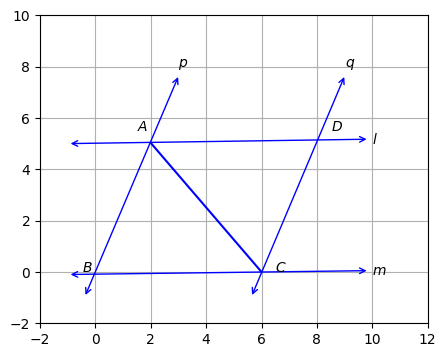
\includegraphics{fig/em1.png}
    \caption{Required parallelogram}
    \label{fig:fig:1}
\end{figure}

\textbf{Solution :}
\begin{table}[H]
    \centering
       \begin{tabular}{|c|c|c|}
    \hline
    \textbf{Input Parameters} &\textbf{Description} &\textbf{Value} \\
    \hline
     $\vec{O}$& Center(at origin)&$\vec{0}$\\
     \hline
 $r$ & Radius &1\\
 \hline
 $\theta$&-&$100\degree$\\
 \hline
 $\alpha$&-&$165.4\degree$\\
 \hline
 $\beta$&-&$5\degree$\\
 \hline
  \end{tabular}

    \caption{Table of input parameters}
    \label{tab:tab:1}
\end{table}

\begin{table}[H]
    \centering
    \begin{tabular}{|c|c|c|}
    \hline
        \textbf{Output Parameters} &\textbf{Description} &\textbf{Value} \\
\hline
          $\vec{Q}$ & Point &$\myvec{\cos{\theta_1}\\\sin{\theta_1}}$\\
          \hline
          $\vec{P}$ & Point &$\myvec{\cos{\theta_2}\\\sin{\theta_2}}$ \\
         \hline
          $\vec{R}$ & Point &$\myvec{\cos{\theta_3}\\sin{\theta_3}}$ \\
         \hline
    \end{tabular}


    \caption{Table of output parameters}
    \label{tab:tab:2}
\end{table}  
From $\figref{fig:1}$ between $\triangle ABC $ and $\triangle CDA$
\begin{align}
\cos{\angle BAC} &= \frac{\innpdt{B-A,A-C}}{\norm{B-A}\norm{A-C}}\\
&=\frac{ab\cos{\theta}+b\sin{\theta}}{b\sqrt{a^2-2ab\cos{\theta}+b^2}}\\
&=\frac{17}{\sqrt{29}\sqrt{41}}\\
\cos{\angle ACD} &= \frac{\innpdt{D-C,A-C}}{\norm{D-C}\norm{A-C}}\\
&= \frac{b^2-ab\cos{\theta}}{b\sqrt{a^2-2ab\cos{\theta}+b^2}}\\
&=\frac{17}{\sqrt{29}\sqrt{41}}\\
So,\angle BAC = \angle ACD.\\
\cos{\angle ACB} &= \frac{\innpdt{B-C,A-C}}{\norm{B-C}\norm{A-C}}\\
&=\frac{a^2-ab\cos{\theta}}{a\sqrt{a^2-2ab\cos{\theta}+b^2}}\\
&=\frac{24}{6\sqrt{41}}\\
\cos{\angle} CAD &= \frac{\innpdt{A-D,A-C}}{\norm{A-D}\norm{A-C}}\\
&=\frac{a^2-ab\cos{\theta}}{a\sqrt{a^2-2ab\cos{\theta}+b^2}}\\
&=\frac{24}{6\sqrt{41}}\\
So,\angle ACB = \angle CAD.
\end{align}
And $CA$ is common side .

So,$\triangle ABC \cong \triangle CDA.\brak{by A-A-S}\brak{proved}$
\end{document}

